%%%%%%%%%%%%%%%%%%%%%%%%%%%%%%%%%%%%%%%%%%%%%%%%%%%%%%%%%%%%%%%%%%%%%%%%%%
%%%%%%%%%%%%%%%%%%%%%%%%%%%%%%%%%%%%%%%%%%%%%%%%%%%%%%%%%%%%%%%%%%%%%%%%%%
\clearpage{}
\section{Systematic uncertainties}
\label{sec:sys}
% ---- ---- ---- ---- ---- ---- ---- ---- ---- ---- ---- ---- ---- ---- ----
\subsection{$W\gamma$+jets normalization uncertainties}
The normalization of the $W\gamma$+jets background is described in
section~\ref{sec:Kfact}. The resulting uncertainties are 6.7\% and
7.9\% for muon and electron channels, respectively.

\subsection{Photon related uncertainties}
In order to estimate the systematic uncertainty in the photon fake rate,
two separate contributions are considered - the effect of biasing the
fake photon template, and the statistical uncertainty in the bias
measurement. The known bias is that the fake photon template is
constructed using inverted PF isolation in the 2012 photon tight selection
ID, where it is assumed that all photon candidates filling this template
are in fact jets faking a photon.

To test this bias, a MC sample
containing jets misidentified as photons is used (such as W+jets MC), along with its
generator information for all jets and photons, to construct the truth
and estimate templates. The muon channel of the MC is used for this study
in order to remove the photon-faking electron contribution. The generator information 
is used to remove all ISR/FSR
photons from the pool of 2012 tight photon candidates in the MC, leaving only
those photon candidates that must be jets misidentified as photons - these will
fill the truth template. The estimate template is filled using the aforementioned
inverted isolation procedure for all photon candidates in the MC. Figure~\ref{fig:para_closure}
demonstrates the shape of both the MC truth and estimate templates, where the
estimate template has been normalized to the truth template using the sideband region of 
$\sigma_{I\etaI\eta} > 0.012$; also, it shows MC shapes compared to the data shapes that are used
in determining the fake rate. The two
templates are compared using the same prescription described for the data-driven
fake rate estimate of the prompt and fake photon templates; however, due to low
statistics in MC after removing all prompt photons, the entire photon $p_{T}$ range
is used to fill one truth template and one estimate template. Any deviation from a
100\% match between the true and estimate templates is considered to be the
measurement of the bias. The bias is measured to be -6\% $\pm$ 11\%, or that the
truth and estimate templates are in 94\% agreement. The uncertainty in this measurement
is included in the overall systematic uncertainty in the fake rate.

\begin{figure}[]
  \begin{center}
    \subfigure[]{
    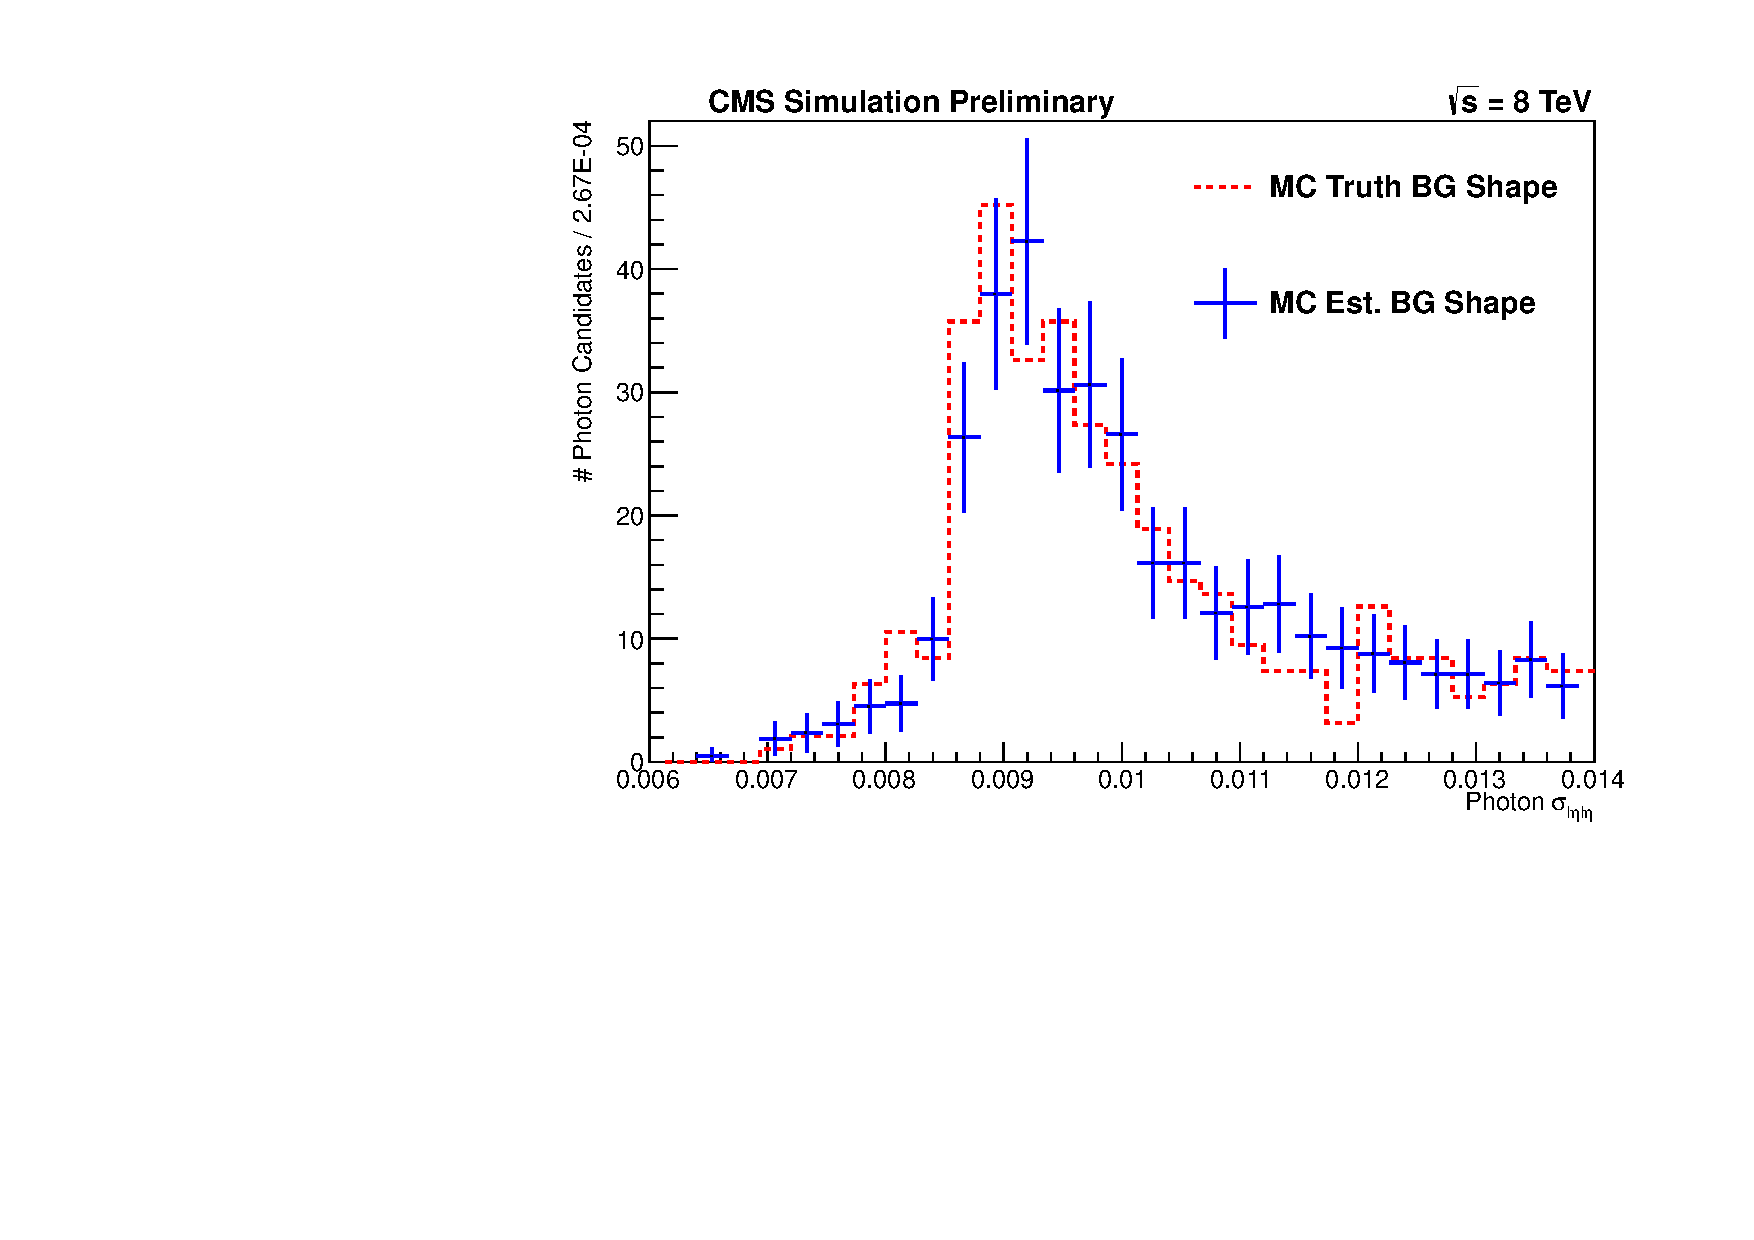
\includegraphics[width=0.5\textwidth]{figs/fakerate_closure.pdf}
  }
    \subfigure[]{
    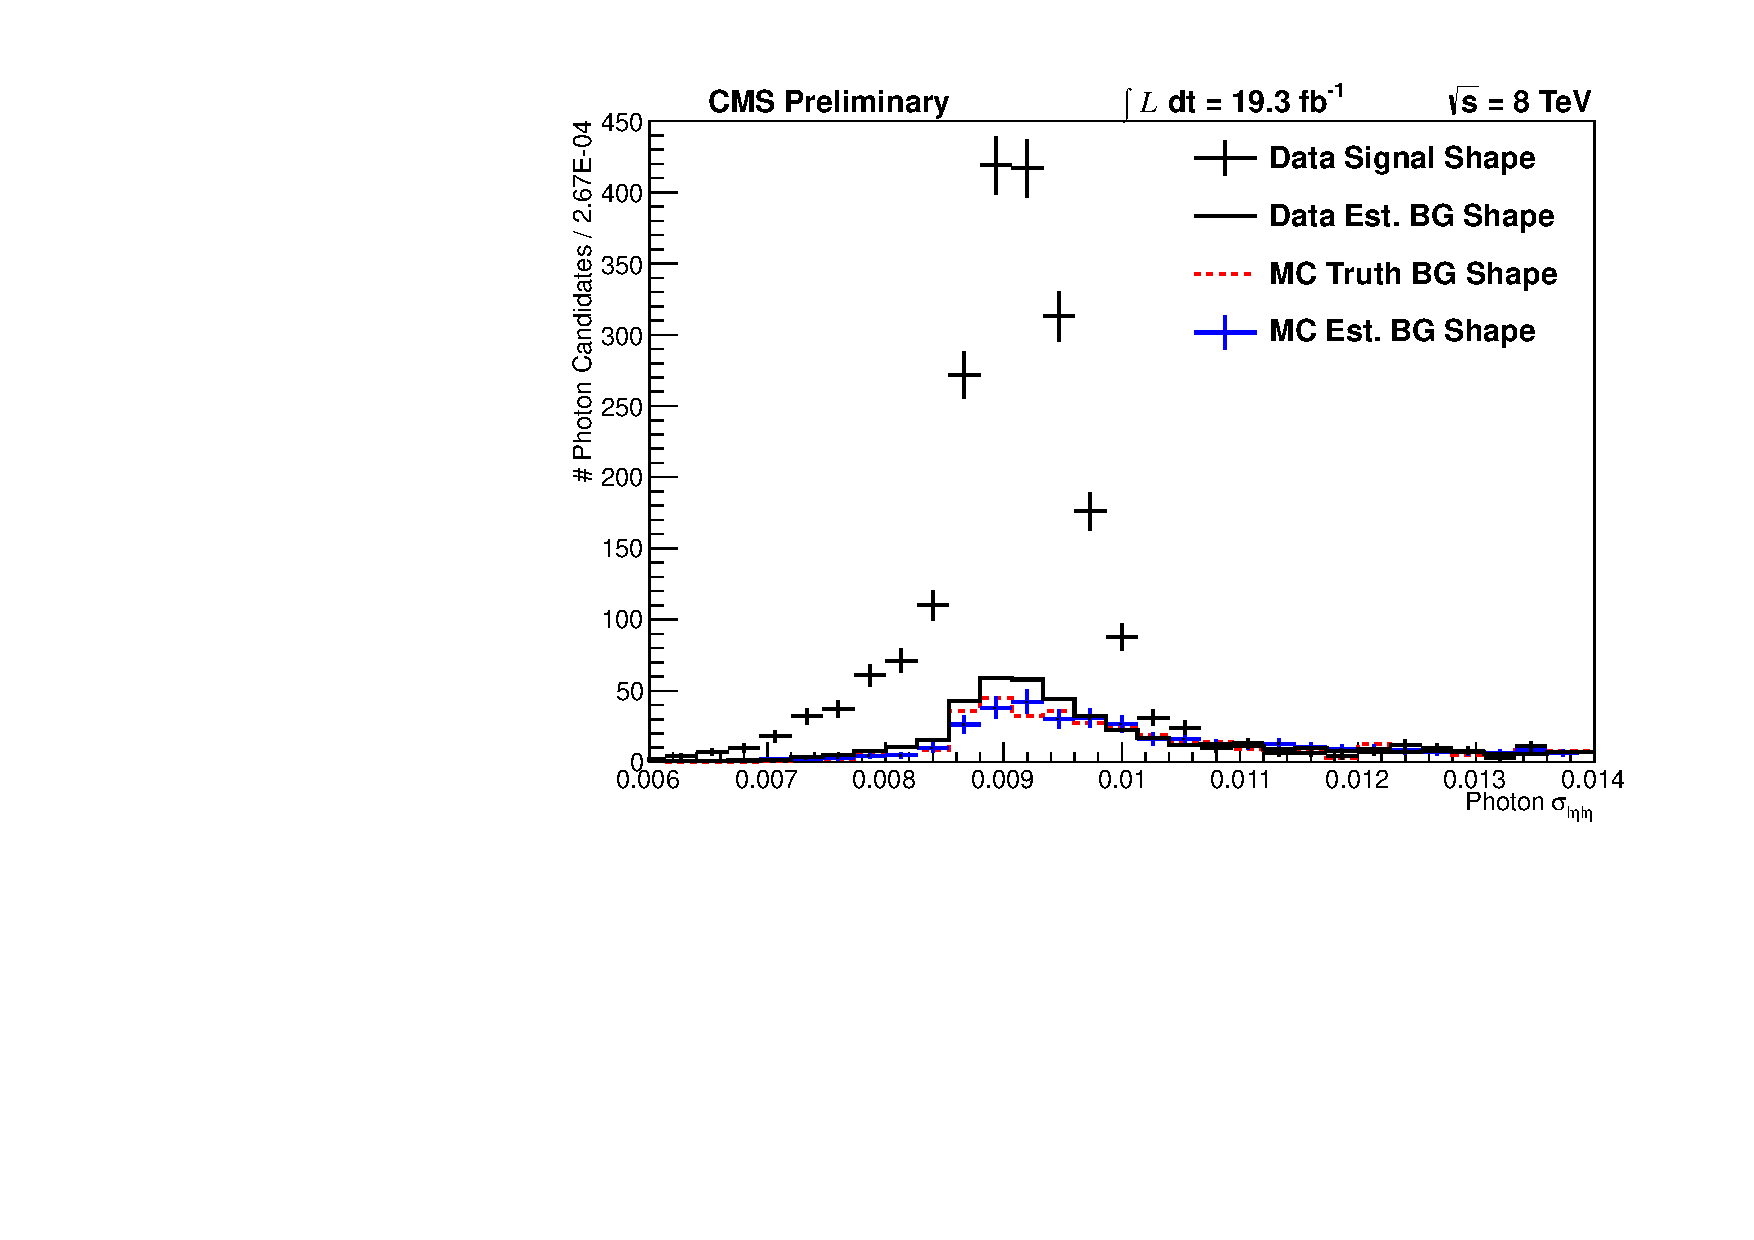
\includegraphics[width=0.5\textwidth]{figs/fakerate_closure_data.pdf}
  }
    \caption{Templates for entire photon $p_{T}$ range (30-400 GeV) for (a) MC Truth versus Estimated photon-faking jet background distribution shapes from the muon channel of a W+3 Jets MC. (b) MC photon-faking jet background distribution shapes compared with data's signal (all 2012 tight photon candidates) and background (photon-faking jets) shapes. The MC Truth template has removed all ISR/FSR photons, while the Estimated templates are filled using the fake rate ratio method utilizing inverted photon isolation.}
  \label{fig:para_closure}
  \end{center}
\end{figure}

The photon $p_{T}$-dependent statistical uncertainty is estimated using toy MCs -
histograms filled with similar statistics as those of the data-driven fake photon
templates, using a random filler. The toy MC histograms
are then treated as the new fake photon templates, while still using the data-driven
prompt photon templates, and the fake photon rate is
remeasured. The RMS of the measurement of the fake rate for all toy MCs is made
the statisticly-driven uncertainty in the fake rate systematic uncertainty. Table~\ref{tab:fakerate_unc}
contains the photon $p_{T}$-dependent statistical uncertainties in the fake rate. 
The measured systematic and statistical uncertainties are combined to make the photon 
$p_{T}$-dependent systematic uncertainties listed in Table~\ref{tab:sys_unc}.


\subsection{ HLT and lepton selection uncertainties}
Systematic uncertainties in the trigger efficiencies are of the order of 1\%. Systematic uncertainties 
in the lepton reconstruction and identification efficiency scale factors are of the order of 2\%.
These uncertainties are accounted for in the final systematics that are input to the limit setter.

\subsection{ \MET uncertainties}
\MET directly affects our signal acceptance. The uncertainty prescription is discussed in \cite{METunc}.
In addition, the \MET distribution in the data is $~3\%$ wider than the MC, and placing a hard
$\MET> 35.0$ cut creates an uncertainty. We estimate it by smearing the \MET for each event by
a Gaussian with a $\sigma = 0.03.\MET$ and observing how many events pass the cut. Specifically,
(Events Passing After Smearing)/(Events Passing Before Smearing) =0.998 for both muons and
electrons.

\subsection{Jet energy scale uncertainties}
The systematic uncertainty is estimated by varying up and down the jet energy uncertainties and computing the effect on the acceptance.
The jet energy scale uncertainty for $pt=30 GeV/c$ in the central region for AK5 PF jets is about $3.5\%$ \cite{CMS-DP-12-012} wich results in $4.3\%$ uncertainty on the 
acceptance.
 
\subsection{ b-tag uncertainties}
The uncertainty from the b-jet CSVM tagging algorithm is
2\% on the data/simulation efficiency correction factor, and is based
on measurement with 2012 data, as described in \cite{CMS-AN-12-470}.
This uncertainty propagated through the analysis has an effect of 11\%
on the $t\overline{t}\gamma$ background, 5\% on the single top
background, and negligible effect on the signal.

\subsection{Pile-up uncertainties}
The average number of pile-up interaction in a given bunch crossing
BX$_{i}$ is given by the following formula:
\begin{equation}
N_{i} = \frac{\mathcal{L} \cdot \sigma_{\textnormal{min. bias}}}{\nu_{\textnormal{orbit}}},
\end{equation}
where $\mathcal{L}$ is the instantaneous luminosity,
$\sigma_{\textnormal{min. bias}}$ is the cross-section of minimum bias
interactions and $\nu_{\textnormal{orbit}}$ is the LHC orbit frequency
(11246~Hz).  Source of uncertainties in the estimation of the number
of pile-up interactions in data then come from the uncertainty on the
luminosity, currently $\textnormal{syst}_{\textnormal{lumi}}=4.4\%$ and
the uncertainty on the minimum-bias cross-section. We have adopted
$\sigma_{\textnormal{min. bias}}=69.3$~mb.

A total variation of 5\% in the number of interactions was propagated to the
re-weighting procedure for signal samples, and the obtained variation
in the signal yield is used as systematics on the signal. The typical
effect is less than a percent.


\subsection{PDF and renormalization/factorization scale uncertainties}
PDF, renormalization and factorization scale uncertainties are described in details in section~\ref{sec:Kfact}.

\subsection{Uncertainties related to the choice of fragmentation model}
The effect on the efficiency for signal due to changes in the dijet mass distribution based on changes in the fragmentation models (Pythia and
Herwig) is investigated. Two MC ttbar sampleas are used, with following changes to the selection:
\begin{itemize}
\item photon selection is removed to gain statistics.
\item events with 2 b-tagged jets and 2 anti-b-tagged jets (CSVM) with $p_{T}>30$ GeV and $|eta|<2.4$ are selected
\item di-jet mass is constructed from the 2 anti-b-tagged jets.
\item di-jet mass distributions are compared in $0<m_{jj}<200$ GeV mass window.
\item fraction of events in $70<m_{jj}<200$ normalized to $0<m_{jj}<200$ region is computed. For the sample, which uses Pythia this fraction is 0.4866 and
for Herwig - 0.4886.
\end{itemize}

The number of events in the sample that pass the modified selection
requirement is about 35000 for the Pythia sample and about 55000 for
Herwig sample.  Comparison for the $m_{jj}$ between the two samples is
shown on Figure \ref{fig:PvsH}.  We conclude that choice of the
fragmentation models (Pythia and Herwig) result in vanishing
systematic uncertainty on the efficiency for signal.

\begin{figure}[b]
  \begin{center}
    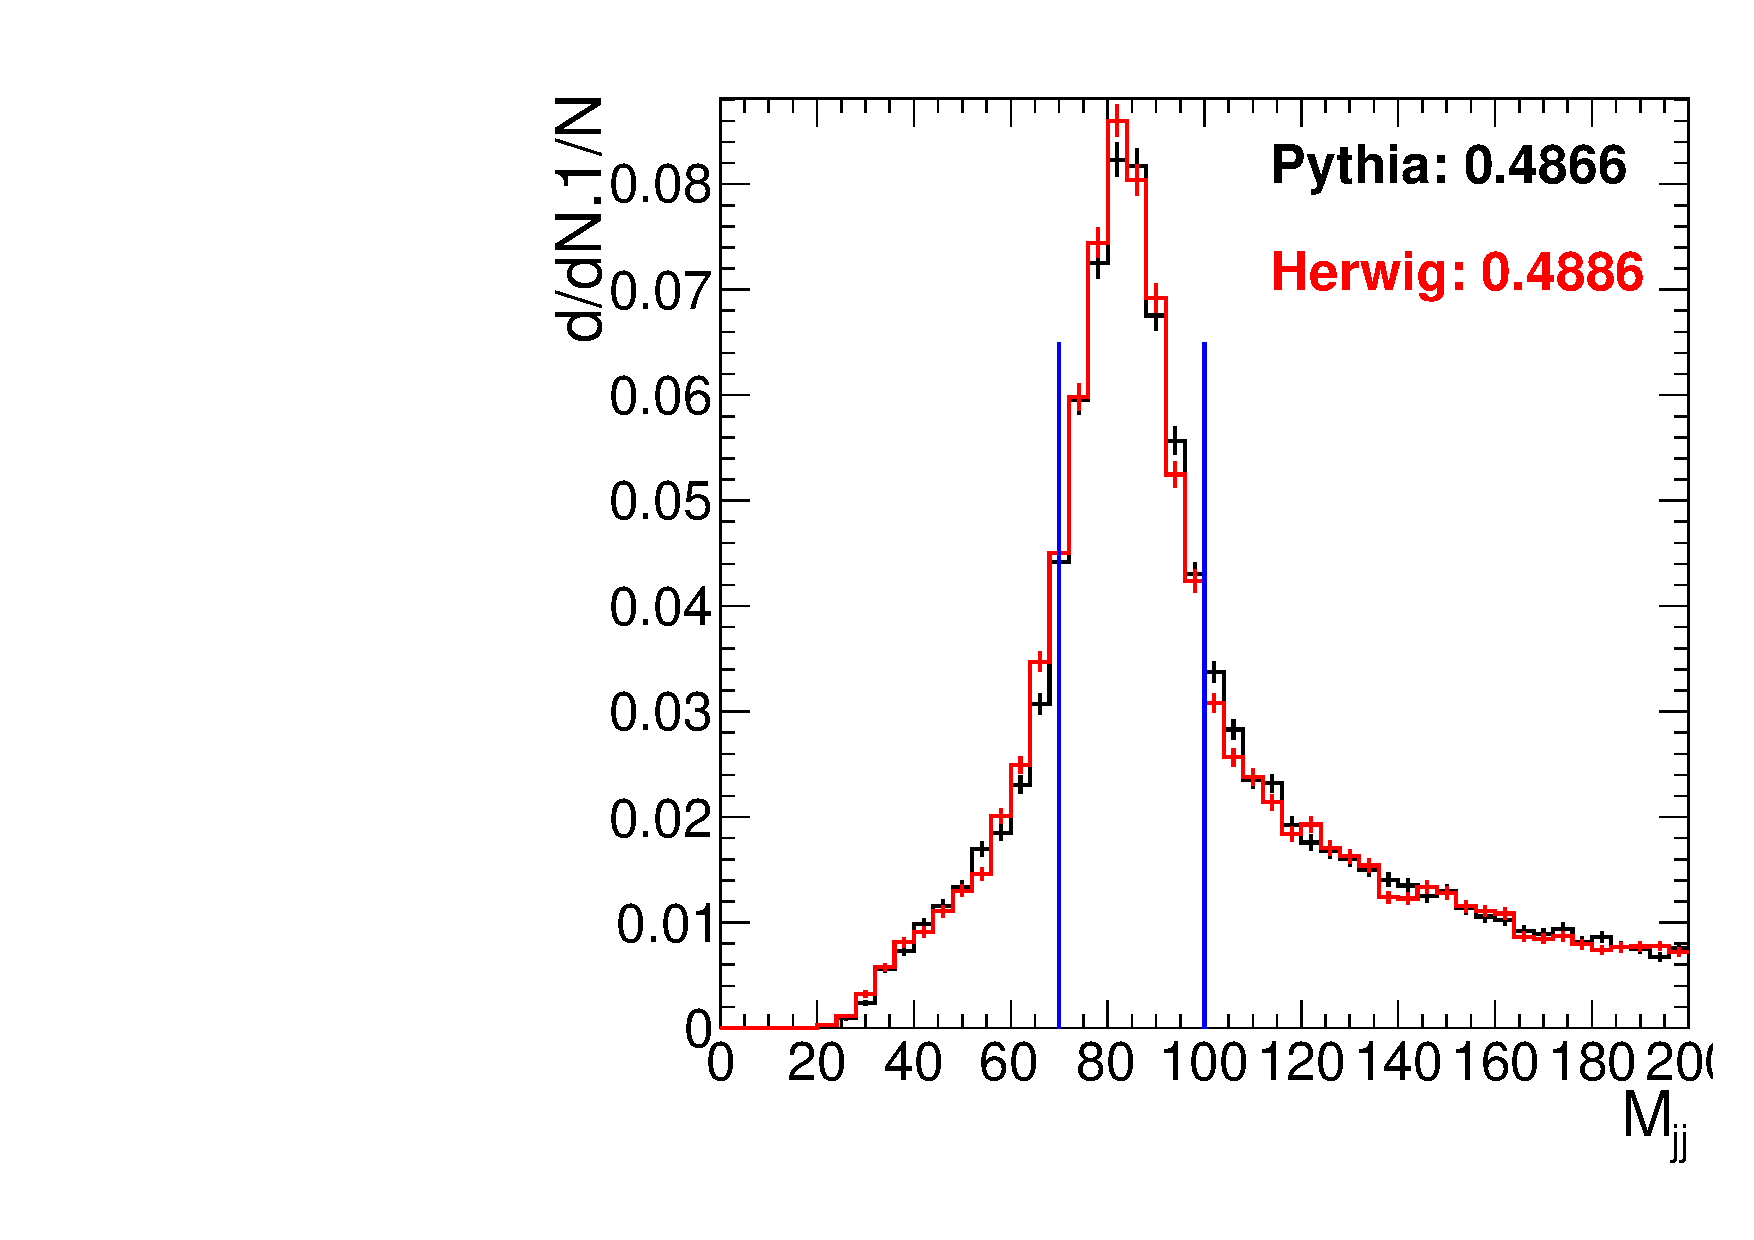
\includegraphics[width=0.42\textwidth]{figs/Pythia_vs_Herwig_Mjj.pdf}
    \caption{ Di-jet invariant mass distribution comparison for samples, produced with different parton showering models: Pythia and Herwig.}
    \label{fig:PvsH}
  \end{center}
\end{figure}


\subsection{MVA selection uncertainty}
We approximated the MVA selection uncertainty with $10\%$ estimate, described in ~\cite{CMS-AN-12-224}. That estimate is based on validation with alsmost pure ttbar 
sample and reflects the largest estimated uncertainty in the ensemble of MVAs, used for a different mass points. In $WV\gamma$ channel the ttbar+gamma yield is 
significantly lower and doesn't allow precise estimation of the systematics. We are in process of evaluation the MVA selection systematic with the moving shapes method.  

\subsection{Systematic uncertainties summary}
In addition, we include the uncertainties described in the companion diboson analysis~\cite{CMS-AN-12-224}, 
as shown in Table~\ref{tab:sys_unc}, as well as uncertainties in the K-factors described in section~\ref{sec:Kfact} 
and photon efficiency scale factors listed in Table~\ref{tab:photon_eff}.  
For the electron channel's QCD contribution, we approximate the systematic uncertainty to be 50\%.

\begin{table}[htb]
\centering
\scalebox{1.15}{
  \begin{tabular}{|c|c|}
  \hline
  Source                        & Uncertainty \\
  \hline
  \hline
  W$\gamma$ + jets normalization  & 6.7\%(mu), 7.9\%(el)       \\
  jet$\rightarrow \gamma$       & 12\% (30 GeV - 50 GeV)  \\
                                & 14\% (50 GeV - 75 GeV) \\
                                & 23\% (75 GeV - 90 GeV) \\
                                & 22\% (90 GeV - 135 GeV) \\
                                & 39\% ($>$ 135 GeV) \\
  multijets                     & 50\%        \\
  \hline
  Trigger Efficiency            & 1\%         \\
  Lepton Selection Efficiency   & 2\%         \\
  Photon Reco/ID Efficiency     & $<$0.5\%      \\
  Jet Energy Resolution         & 1\%         \\
  Jet Energy Scale              & 4.3\%         \\
  Photon Energy Scale           & 1\%         \\
  \MET                          & 1\%         \\
  Anti-b Tag ($t\overline{t}\gamma$)  & 11\%        \\
  Anti-b Tag (single top + $\gamma$)  & 5\%         \\
  Pileup modeling               & 1\%         \\
  \hline
  renormalization/factorization scale                   & 23.4\%         \\
  PDF                           & 3.6\%         \\
  \hline
  Luminosity                    & 4.4\%         \\
  \hline
  \end{tabular}}
  \caption{Summary of the systematic uncertainties.}
  \label{tab:sys_unc}
\end{table}

